\documentclass[conference]{IEEEtran}

  \usepackage{booktabs}
  \usepackage{listing}
  \usepackage{amsmath}
  \usepackage{algorithm}
  \usepackage{array}
  \usepackage{url}
  \usepackage{cite}
  \usepackage{complexity}
  \usepackage{algpseudocode}
   \usepackage{graphicx}
   \usepackage{enumerate}
   \usepackage{subcaption}
   \usepackage[shortlabels]{enumitem}


% \usepackage{algorithm}
  \ifCLASSINFOpdf
  
  \else
  
  \fi
  
  \hyphenation{op-tical net-works semi-conduc-tor}
  
  \begin{document}
  
  \title{Elite Parent Preserving Evolutionary Neural Architecture Search for Image Classification \\ Final Report}
  
  \author{\IEEEauthorblockN{Bowen Zheng, Shijie Chen, Shuxin Wang}
  \IEEEauthorblockA{Department of Computer Science and Engineering\\
  Southern University of Science and Technology\\
  Shenzhen, Guangdong, China\\}
  }
  
  \maketitle
  
  \begin{abstract}
  In this project, we propose an elite-parent preserving evolutionary framework for Neural Architecture Search on image classification problems. We have finished the evolutionary algorithm framework and the construction of neural architecture. Currently we focus on a cell-based search space where a neural architecture is composed of multiple interconnected cells. Experiments show the effectiveness of our algorithm in obtaining a neural architecture with good performance. In the future, we will try to improve the effectiveness of mutation operations and efficiency of training new individual networks.
  
  \end{abstract}
  \IEEEpeerreviewmaketitle
  
  \section{Introduction}
      The great leap of computing resources in the past few decades made it possible to fully utilize the potential of neural networks. In recent years neural networks outperformed traditional methods in many fields of research, especially image classification. However, the state-of-the-art architectures are carefully designed and tuned by researchers for a specific problem. Therefore, people start to think about automating the design of neural networks in the hope of finding the best-performing network architecture efficiently.

      Neural architecture search is a research field focusing on automating the design of neural networks. Currently there are a few popular approaches, including reinforcement learning, Bayesian optimization, tree-based searching and genetic-based evolutionary algorithms. 

      This project focuses on NAS for image classification problems. The reason is that this area is well explored and there exist many high-performance hand-crafted neural architectures. They provide a good guidance and target to our project. In addition, neural networks for image classification are mostly built upon basic units including convolution, polling, normalization, and activation layers. This helps to shrink our search space.
    


    \section{Related Works}
    A lot of research works have been done on NAS. Some researchers have proposed algorithms that can design architectures with performance on par of or even better than state-of-the-art hand-crafted neural networks. Research topics in NAS are divided into three categories: search space, search strategy and performance estimation strategy.
    
    \subsection{Search Space}
    
    The search space of NAS determines the possible architectures a NAS algorithm can find.

    The simplest search space is the simple multiple-layer structure, in which a neural network $A$ is composed of multiple layers $L_i$ connected to the neighboring layers. In this case, the search space can be described by (1) The maximum number of layers (2) The type and dimension of each layer and their hyper-parameters\cite{chollet2017xception}\cite{baker2016designing}. 

    In more recent studies, some researchers use a cell-based search space in which the possible architecture of cells is explored. A cell is nothing but a smaller neural network. The entire neural network is constructed by connecting several pre-defined cells. A cell has fewer layers but allows more complex architectures like skip connections between any layers\cite{cai2018path}\cite{real2018regularized}. The cell could be some hand-crafted neural networks that have already been proofed effective. The search space is therefore decreased to the possible arrangements of cells.

    In contrast to the above direction, some researchers also tried to search for effective cells and connect them at last in a predefined manner\cite{zoph2018learning}\cite{cai2018path}. The search space is greatly decreased in that each cell is comparably small. This method can also be easily transferred to other datasets\cite{zoph2018learning} since the structure of cells is not fixed.

    Recently, some researchers managed to optimize the overall architecture as well as the cells at the same time and obtained state-of-the-art result\cite{liu2019auto}.
    
    \subsection{Search Strategy}
    
    Many different search strategies can be applied to explore the search space discussed above. These methods include Bayesian optimization, evolutionary methods, reinforcement learning and gradient-based methods. 

    Evolutionary algorithms have been used to evolve neural networks since 1989\cite{miller1989designing}. Earlier works use genetic algorithms to both optimize the structure of neural networks and train the networks\cite{stanley2002evolving}. However, with the birth of back-propagation (BP), recent works of neural-evolution use genetic algorithms only for optimizing neural architectures and use BP to train the networks\cite{real2017large}. In the context of NAS, the individuals in the genetic algorithm are neural network architectures and the genetic operations (crossover and mutation) are used to alter the architecture by adding/removing layers or change the connectivity of nodes.

    Genetic algorithms show their diversity in how they sample parents, generate offspring and update population. Some work choose parents from a preto-optimal front\cite{elsken2018efficient} while others use tournament selection\cite{liu2018progressive}\cite{real2018regularized}\cite{real2017large}. When generating offsprings, some algorithms randomly initialize the weight of child networks. In comparison, Lamarckian inheritance is used in \cite{elsken2018efficient} so that child networks could inherit the weight of its parent and the training cost is reduced. To update population, some algorithms abandon least capable individuals\cite{real2017large} while some delete the oldest individuals\cite{real2018regularized}. A more sophisticated policy is developed by \cite{Hornby:2006:AAP:1143997.1144142} and \cite{DBLP:journals/corr/abs-1802-01548} in which the age of the individuals are taken into account.
    
    There are other methods that are used to implement NAS, including Bayesian optimization, reinforcement learning,tree-based search and gradient-based methods. We don't discuss them here since we use evolutionary algorithms in our project.

    \subsection{Performance Estimation Strategy}
    One important issue in neural architecture search is the estimation of neural network performance. This is critical in the population update policy of evolutionary algorithms. 

    The simplest way to estimate performance is to train every searched network from scratch and test the desired performance metric, e.g. accuracy on the validation set. However, the training of the neural network is very time and computation consuming. 
    
    An alternative is to estimate performance on lower fidelities. More specifically, to train the network for a shorter period of time\cite{zoph2018learning} or on some subset of the dataset\cite{klein2016fast}. However, the estimate must ensure the result ranking of different networks must be the same as that of complete training. That is to say, there exists a trade-off between computational load and estimation fidelity.

    Another approach to estimate performance is based on learning curve extrapolation\cite{domhan2015speeding}. This method accelerates estimation by stop poor performance networks in the early state of training based on statistical patterns of learning curves. Other researchers propose ways to predict neural network performance based on architectural and cell properties\cite{liu2018progressive}. 

    \section{Methodology}

    We will develop an evolutionary neural architecture search algorithm based on the $age$ of individuals. By incorporating $age$ as a part of a gene, we can prolong the existence of good individuals\cite{DBLP:journals/corr/abs-1802-01548} and kill average individuals when their age reaches a certain limit\cite{Hornby:2006:AAP:1143997.1144142}. 

    Combining the advantage of the above works, we propose a population update police based on $age$ and that preserves a parent whose child has good performance. An individual is dropped from the total population if its $age$ exceeds a predefined $lifetime$. However, we prolong its life if its offspring performs well (e.g. within top $P\%$ in ranking). In this way, we hope to preserve good parent architectures in the population.

    To test the effectiveness of our algorithm, we will experiment on image classification datasets including CIFAR-10, CIFAR-100 and will possibly extend to IMAGENET.


  \section{System Design}
  \subsection{Cell-based Search Space}

  We explore a cell-based search space with 5 hidden cells, as is illustrated in Fig.\ref{f_artc}. Each edge in Fig.\ref{f_artc} represents a neural network unit. Each square represents a tensor in the neural network.

  \subsubsection{Neural Network Units}
  
  There are 7 possible neural network units that are suitable for image classification problems in our search space:

      \begin{enumerate}
        \item identity
        \item $3\times3$ average polling
        \item $3\times3$ max polling
        \item $1\times1$ convolution
        \item $3\times3$ depthwise-separable convolution
        \item $3\times3$ dilated convolution
        \item $3\times3$ convolution
      \end{enumerate}

  The search space is the possible connections of the states using different neural network units.

  \subsubsection{Cell Architecture Representation}

  We represent the architecture of a cell by a vector $R$ which is a vector of lists of tuple $R_{i} = \{(a_{i1}, b_{i1}), (a_{i2}, b_{i2}), ...\}$ where $a_i$ marks the input state of state $i$ and $b_i$ shows the unit used in the state transition connection.

  \begin{figure}[H]
     \centering
     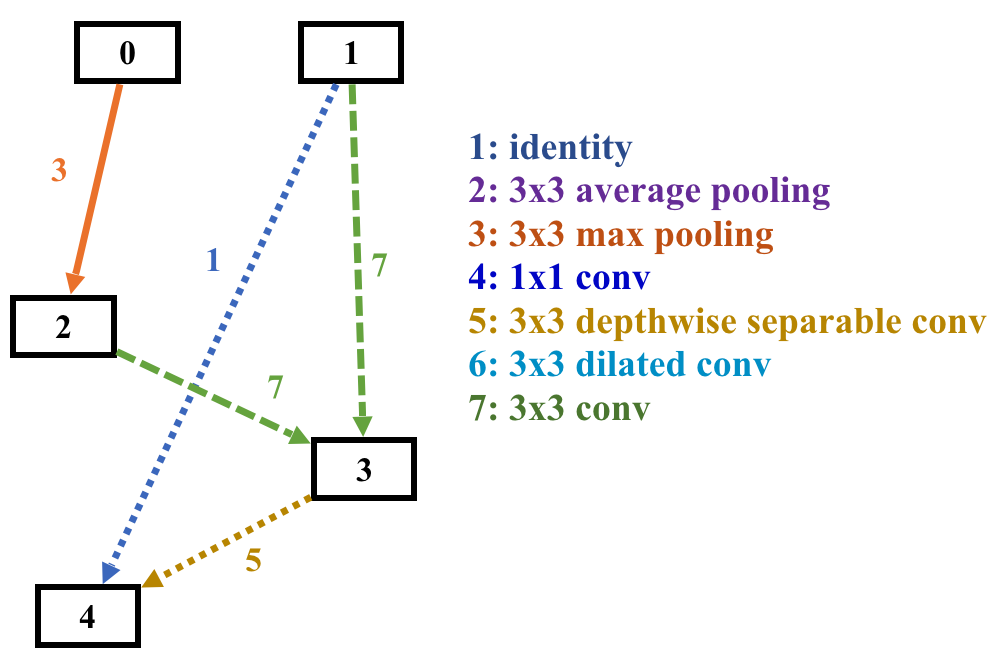
\includegraphics[width=0.4\textwidth]{figures/cellStruct.png}
   \caption{An example artitecture of a cell with representation $R=\{\{\},\{\},\{(0,3)\},\{(2,7),(1,7)\},\{(1,1),(3,5)\}\}$.}\label{fig:digit}
   \label{f_artc}
  \end{figure}

  \subsection{Overall Neural Network Architecture}
  We use an architecture similar to \cite{He_2016_CVPR} to obtain a good performance. As is illustrated in Fig.\ref{total_artc} overall network consists of input layer, 6 ($N = 2$) identical cells, 3 polling layers, 1 global average polling(GAP) layer, 2 fully connected(FC) perceptron layers and 1 softmax layer. 

  \begin{figure}[H]
     \centering
     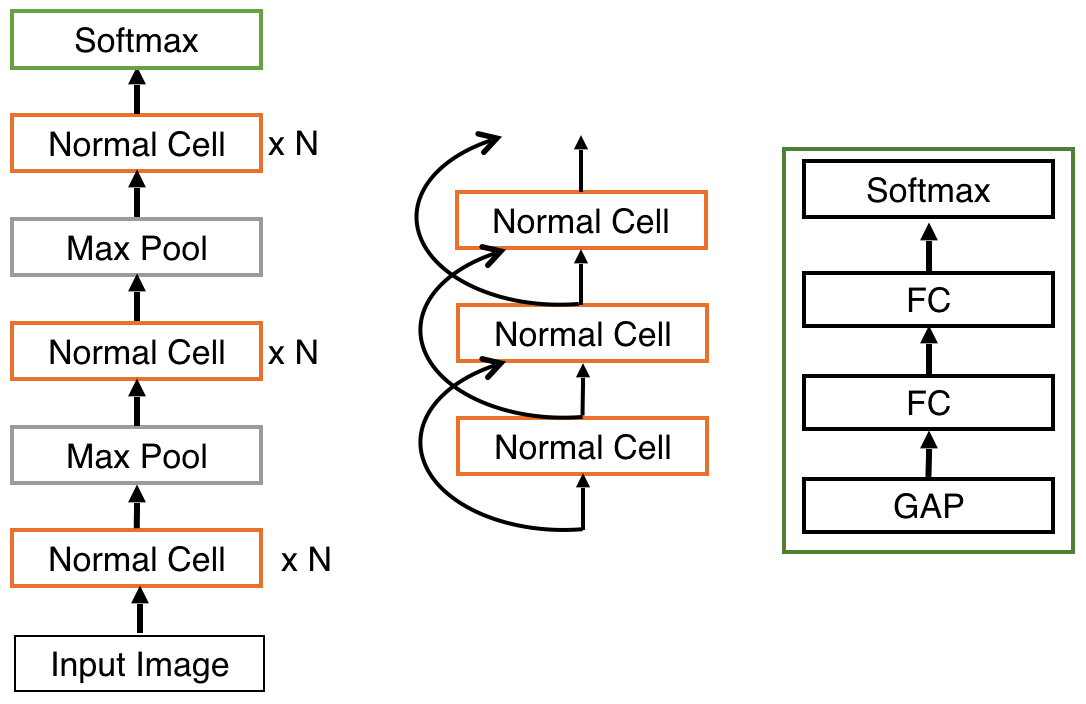
\includegraphics[width=0.4\textwidth]{figures/overallStruct.png}
   \caption{The simplified overall artitecture of the total network. LEFT: outer structure. MIDDLE: detailed structure of normal cell stack. RIGHT: detailed structure of the Softmax unit.}\label{fig:digit}
   \label{total_artc}
  \end{figure}

  For simplicity, all cells share the same structure.
  
  

  \subsection{Early Stop Performance Estimation}

  To accelerate the evolution process, we need to find a way to estimate the performance of a generated neural architecture. We use an early-stop strategy that trains the neural network with a small \emph{epoch} value. This approach can noticeably cut the training time of a network and at the same time provides a relatively reliable performance comparison metric.

  \subsection{Evolutionary Algorithm Framework}
  
  \begin{algorithm}[H]  
    \caption{ Elite Parent Preserving Evolution}
    \begin{algorithmic}[1]  
  
    \State $population\gets \phi$
    \State $entireGen\gets \phi$
    \State $generation\gets 0$
    
    \While{$population$ size$<N$}
    \State $newNetwork\gets networkInit()$
    \State $trainNetwork(newNetwork)$
    \State add $newNetwork$ to $popution$ and $entireGen$
    \EndWhile
    
  
    
    \While {$genetation < G$}
      \State $parent\gets$ select a parent from population using tournament selection 
      \State $child \gets mutate(parent)$
      \State $trainNetwork(child)$
      \State add $child$ to $popution$ and $entireGen$
      \If {accuracy of $child$ is better than $P\%$ individuals in population}
        \State extend the $lifetime$ of $parent$ by $t$
      \EndIf
      
      \ForAll {$individual$ in $population$}
        \State update the $age$ of $individual$
        \State remove current $individual$ if its $ age $ reaches its $lifetime$
      \EndFor
      
      
    \EndWhile
    
    
    \\  
    \Return the network model with highest accuracy in $entireGen$
 
  \end{algorithmic}  
  \end{algorithm}  
  For now, we follow the design of a cell based evolutionary NAS algorithm described in\cite{DBLP:journals/corr/abs-1802-01548} except that we propose a population update policy to preserve good parents. 
  Our evolutionary algorithm features an elite parent preserving strategy in which the lifetime of the parent whose child has a high accuracy rank within the total population is extended. In this way, we hope to preserve good genes in the population and produce more high-quality offsprings.

The $population$ size is $N$ and the algorithm evolves $G$ generations in total. $entireGen$ stores all network models that we generated. $P$ and $t$ are hyper-parameters controlling the actual lifespan of an individual.
     

In our midterm experiment, we use Network Initialization ver.1 to generate the initial network. New networks are generated with a random architecture. In the meantime, their $age $ being set to 1 and $lifetime$ being set to the default value. Besides, their accuracy will be estimated right after they being generated.
 \begin{algorithm}[H]  
    \caption{ Network Initialization ver.1}
    
    
    \begin{algorithmic}[1]  
        \Ensure A randomly generated network.
    \State $network\gets $ new $Network$
    \State $network.age\gets1$
    \State $network.life\gets $DEFALT\_LIFE 
    
    \State $arch\gets \phi$

    \ForAll  {$l$ in hidden layers } 
    \State $edge_l \gets \phi$
    \For {every input layers and hidden layers before $l'$}
    \If{$random<p$}
    \State $e \gets$ edge from $l'$ to $l$ with an randomly chosen neural network unit.
    \State $edge_l$.add($e$)
    \EndIf
        \EndFor

        \If{in-degree of $l>$0}
        \State  $e \gets$ legal edge to $l$ with a random unit.
        \State $edge_l$.add($e$)
        \EndIf
    \State $arch$.add($edge_l$)
        \EndFor
    
    \State $edge_{out} \gets \phi$
    \ForAll {$i$ with 0 out-degree}
      \State $e \gets$ edge from $i$ to output layer with identity unit.
      \State $edge_{out}$.add($e$)
    \EndFor

    \State $arch$.add($edge_{out}$)
    \State $network.arch=arch$
    \State $network.accuracy\gets getAcc()$
    \\
        \Return The $network$ generated.
        
    \end{algorithmic}  
\end{algorithm}  


However, we find it is inefficient to initialize population in this way. After receiving some advice from prof. Ishibuchi, we decided to initialize and evolute our population based on one or several existing network architecture with good performance.

In our current experiment, we based on the ResNet Architecture in Fig.\ref{resnet}. Our network initialization algorithm has also been modified to Network Initialization ver.2.
\begin{figure}[H]
	\centering
	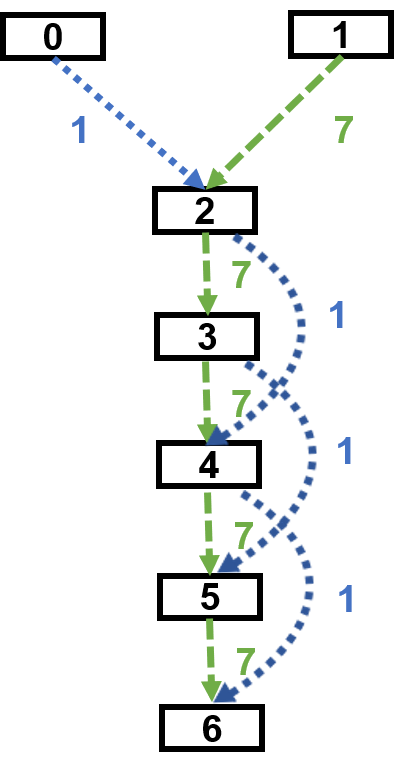
\includegraphics[width=0.25\textwidth]{figures/fig_resnet.png}
	\caption{ResNet Architecture.}\label{fig:digit}
	\label{resnet}
\end{figure}

 \begin{algorithm}[H]  
	\caption{ Network Initialization ver.2}
	
	
	\begin{algorithmic}[1]  
		\Ensure A randomly generated network.
		\State $network\gets $ new $Network$
		\State $network.age\gets1$
		\State $network.life\gets $DEFALT\_LIFE 
		
		\State $arch\gets $ ResNet $ arch$ 
		
		\State $arch\gets HeuristicMutation(arch)$
		\State $network.arch=arch$
		\State $network.accuracy\gets getAcc()$
		\\
		\Return The $network$ generated.
		
	\end{algorithmic}  
\end{algorithm}  

  \subsection{Heuristic Mutation Operators}
  When sampling the parent individuals, we randomly take $X$ individuals from the population and pick the one with the highest estimated accuracy. The mutation operation includes adding, deleting and altering an edge(NN unit). Fig.\ref{mutation} gives an example. At the same time, the resulting model must be valid and conform to our representation definition. 
  

  



 \begin{algorithm}[H]  
	\caption{Heuristic Mutation Operation}
	
	
	\begin{algorithmic}[1]  
		\Require A network architecture $arch$
		\Ensure The $arch$ with a heuristic mutation
		
		\State Randomly pick a mutation operation using the heuristic rule.
		
		\State Randomly pick a proper mutate position between two hidden layer according to the chosen mutation operation.
		
		\State Apply the chosen mutation operation to the position.
		
		\State $edge_{out} \gets \phi$
		\ForAll {$i$ with 0 out-degree}
		\State $e \gets$ edge from $i$ to output layer with identity unit.
		\State $edge_{out}$.add($e$)
		\EndFor
		
		\State $arch$.replace($edge_{out}\_old$,$edge_{out}$)
		
		\\
		\Return arch
	\end{algorithmic}  
	\label{mutation}
\end{algorithm}  

  A heuristic mutation procedure is designed for the evolutionary algorithm. Different weights are given to structure change (connection addition and deletion) and connection change (connection type). At first, we randomly choose a mutation operation using the heuristic rule. Then the mutate position is randomly chosen restricted by the chosen operation(The position should be able to apply such kind of operation). The probability of edge deletion and addition are both $15\%$. The probability of change operation is $70\%$. We also divide connections into two categories: convolutions and pooling operations and assign to them different weight in mutations. More specifically, the probability that an edge becoming a convolution is $80\%$ and that an edge becoming a pooling operation is $20\%$ in connection change. 

\begin{figure}[H]
	\centering
	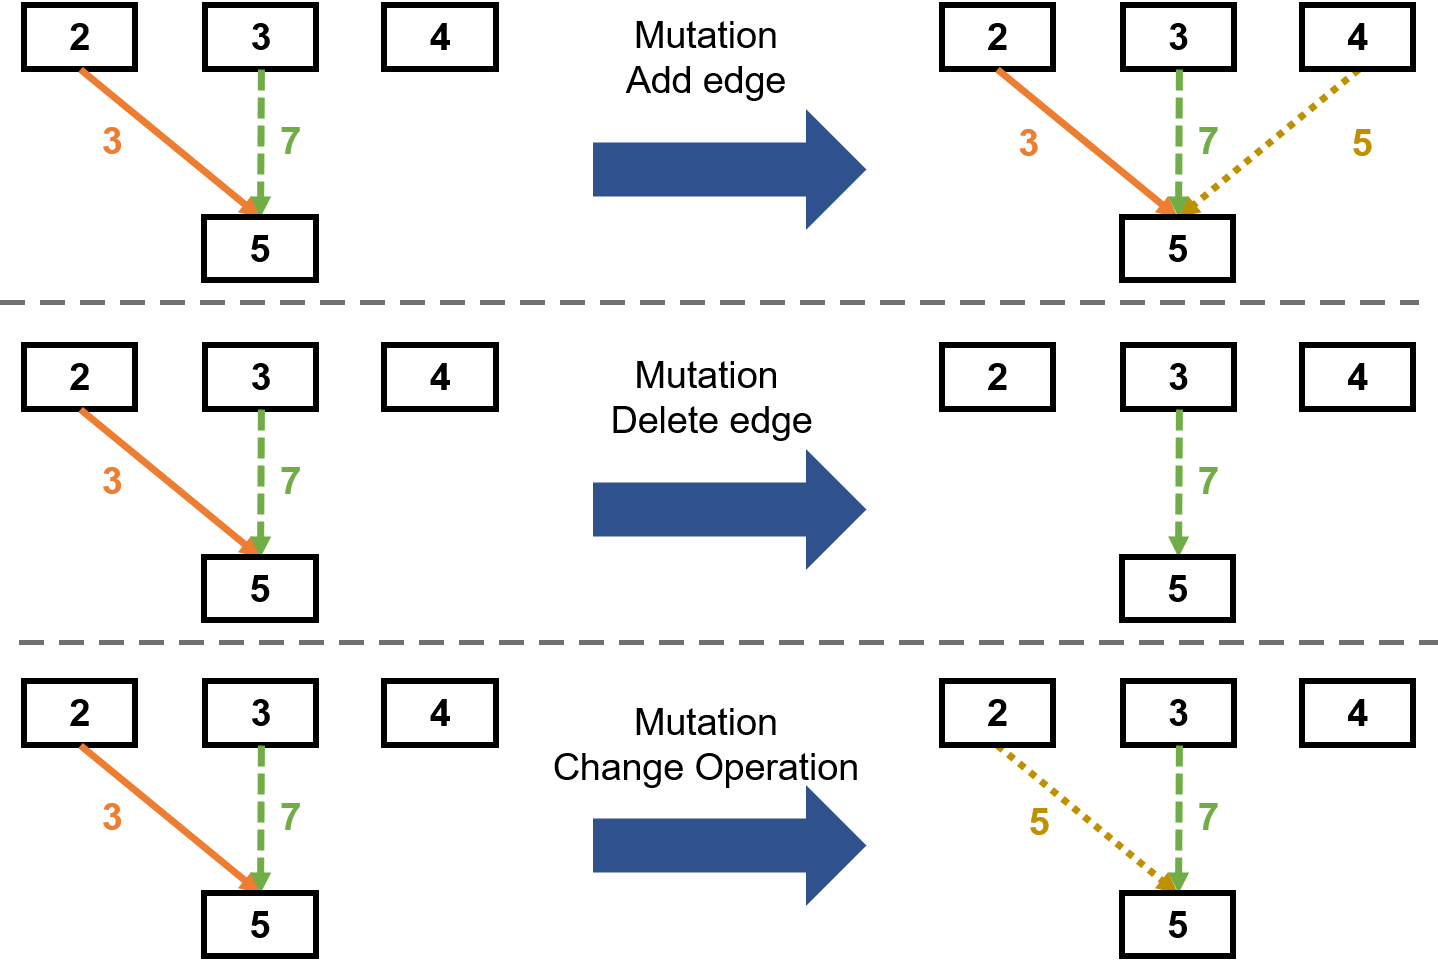
\includegraphics[width=0.45\textwidth]{figures/mutation.png}
	\caption{Three mutation operations.}\label{fig:digit}
	\label{mutation}
\end{figure}


 \section{Experiments}

 \subsection{specification}
 The followings are the parameters used in our experiment during search process.
 \begin{enumerate}
  \item Population Size $population$ = 10
  \item Tournament Size $X$ = 3
  \item Total Generations: 30
  \item Batch Size: 400
  \item Learning Rate: 0.001
  \item Epoch: 50
  \item Stack depth: $N = 2$
  \item Number of Channels: 64 for stack1, 128 for stack2, 256 for stack3 and 512 for stack 4.
  \item Number of Hidden Layers in a Cell: 4
 \end{enumerate}

 \subsection{Result}

 Fig.\ref{found_artc} shows the best model our algorithm found that reaches an accuracy of 76\% on CIFAR-10 dataset.Currently, our model is still primitive. This found model is not fully trained. We expect better performance after a full training.

\begin{figure}[H]
 	\centering
 	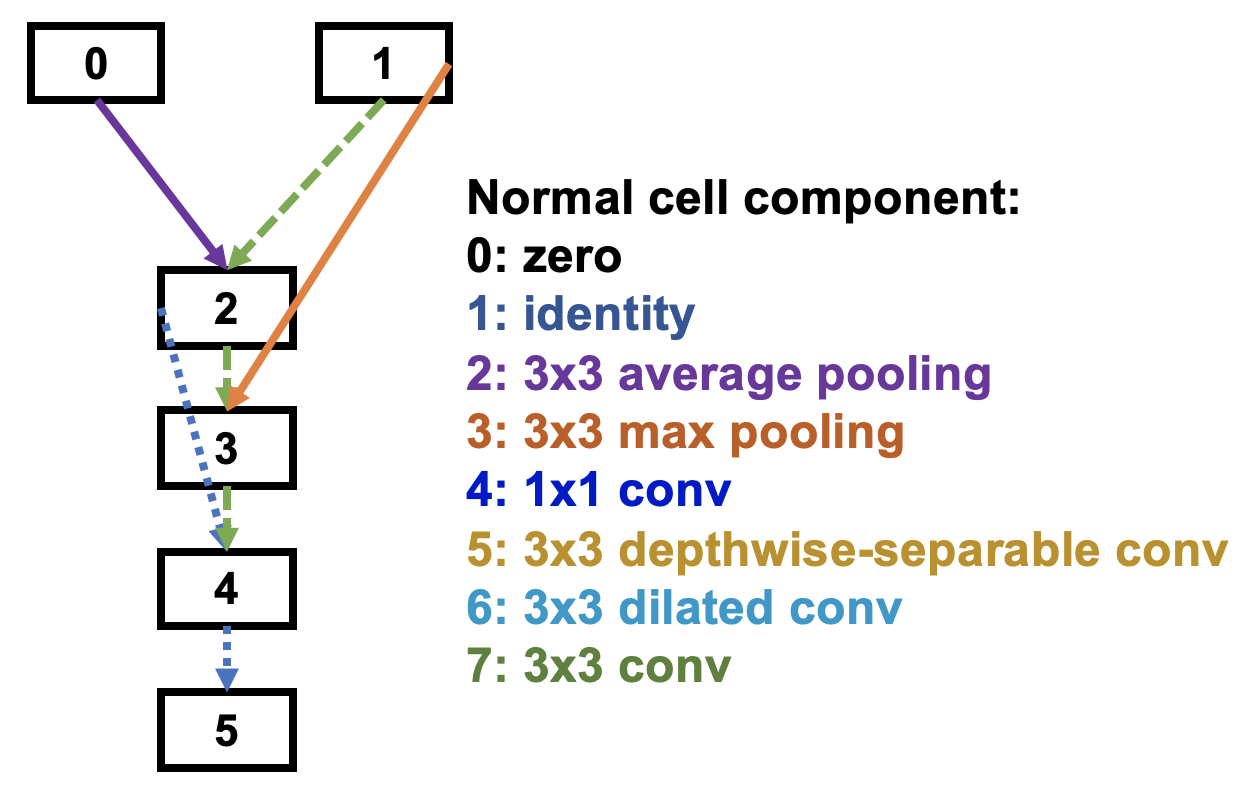
\includegraphics[width=0.4\textwidth]{figures/newResult.png}
   \caption{Structure of the found network. }\label{fig:digit}
   \label{found_artc}
  \end{figure}

\begin{figure}[H]
	\centering
	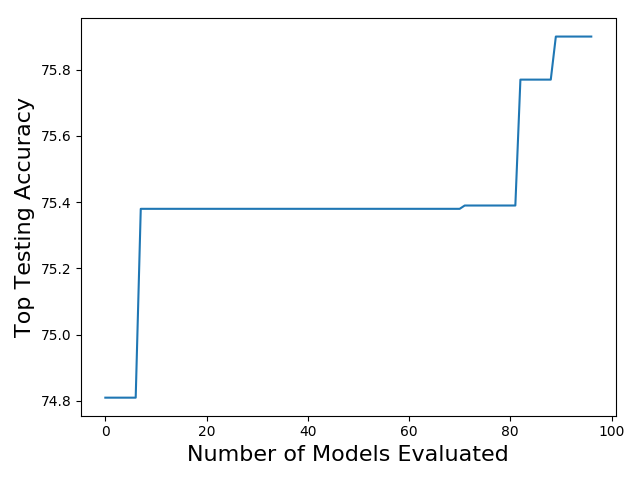
\includegraphics[width=0.45\textwidth]{figures/result_curve.png}
	\caption{Accuracy result.}\label{fig:digit}
	\label{curve}
\end{figure}

\subsection{Analysis}
  Through some experiments, we observe some problems in this project.

  The biggest problem is computational cost. Currently we have not implemented weight sharing between parent and child networks. Therefore, the evaluation of each newly generated networks takes a lot of time. Depending on the capacity of a network, evaluation of a network may some time from half an hour to several hours. This makes it hard to improve the total number of generations in the evolutionary algorithm, limiting the  search ability of our algorithm.

  In addition, our code didn't have good parallelism. This means that currently we can't fully utilize the power of multi-core CPUs and multiple GPUs on a server. Also, we may use some parallel evolutionary algorithms to improve the search ability of our algorithm. For example, running different evolutionary operators on different cores and machines. Improved parallelism can enhance earch ability as well as efficiency of our model.
  
  Besides, we lack some knowledge in the effecttiveness of different structures in a convolution neural network. Our heuristic mutation strategy is still based on simple probability. A better mutation operator can be designed based on graph theory or other domain knowledge about neural networks.



 \section{Future Work}  

 We have already defined the representation of neural architectures and have implemented the evolutionary search algorithm. The following are the improvements we are going to make for finishing this project.
 
  
  \subsubsection{Weight Sharing of Neural Networks}    
  One major cost in NAS is the training of neural networks. Offspring networks are generated through mutation operation and share a lot of structures with their parents. Therefore, we can let the offspring inherit the weights of its parent. This will cut the training time cost significantly compared to training a neural network from scratch.
  
  \subsubsection{Evolutionary Operators}
  Our current mutation strategy depends only on simple probabilities. We may look into the usage of different components in the neural network to find a better mutation strategy.

  Our current model only uses mutation as evolutionary operator. We may also look at some works that focus on crossover operations between neural networks. Hopefully, this will help us improve search ability.

  \subsubsection{More Efficient Performance Estimation}
  A better performance estimation approach is needed to accelerate the search process. We may try some approaches that require little training or can distinguish good neural networks from bad ones efficiently.
   

\bibliographystyle{ieeetr}
\bibliography{ref}
% that's all folks
\end{document}


  